To isolate the different parts of the system and limit overlap between groups, the project was divided in accordance with figure~\ref{fig:architecture} into three parts, frontend, backend and tester.

Frontend was designed to avoid keeping state. By doing so, the user-facing components could scale out to multiple backend servers and keep commonly used content cached. This would allow for better load-balancing where frontends could be geographically distributed and yield lower latencies.

Backend was designed to control the database and to keep a centralized management of state transitions. A feature that was discussed, but not investigated, was to shard the data between backends. That would have allowed even greater flexibility in the development of the platform, should it be used in more than one place.

Since tester could be used by other projects than the Gamified Programming Platform, it was designed to be idempotent and stand-alone. This meant that any tester server would yield the same result every time it was queried and have no prior knowledge of the system.
\begin{figure}
    \centering
    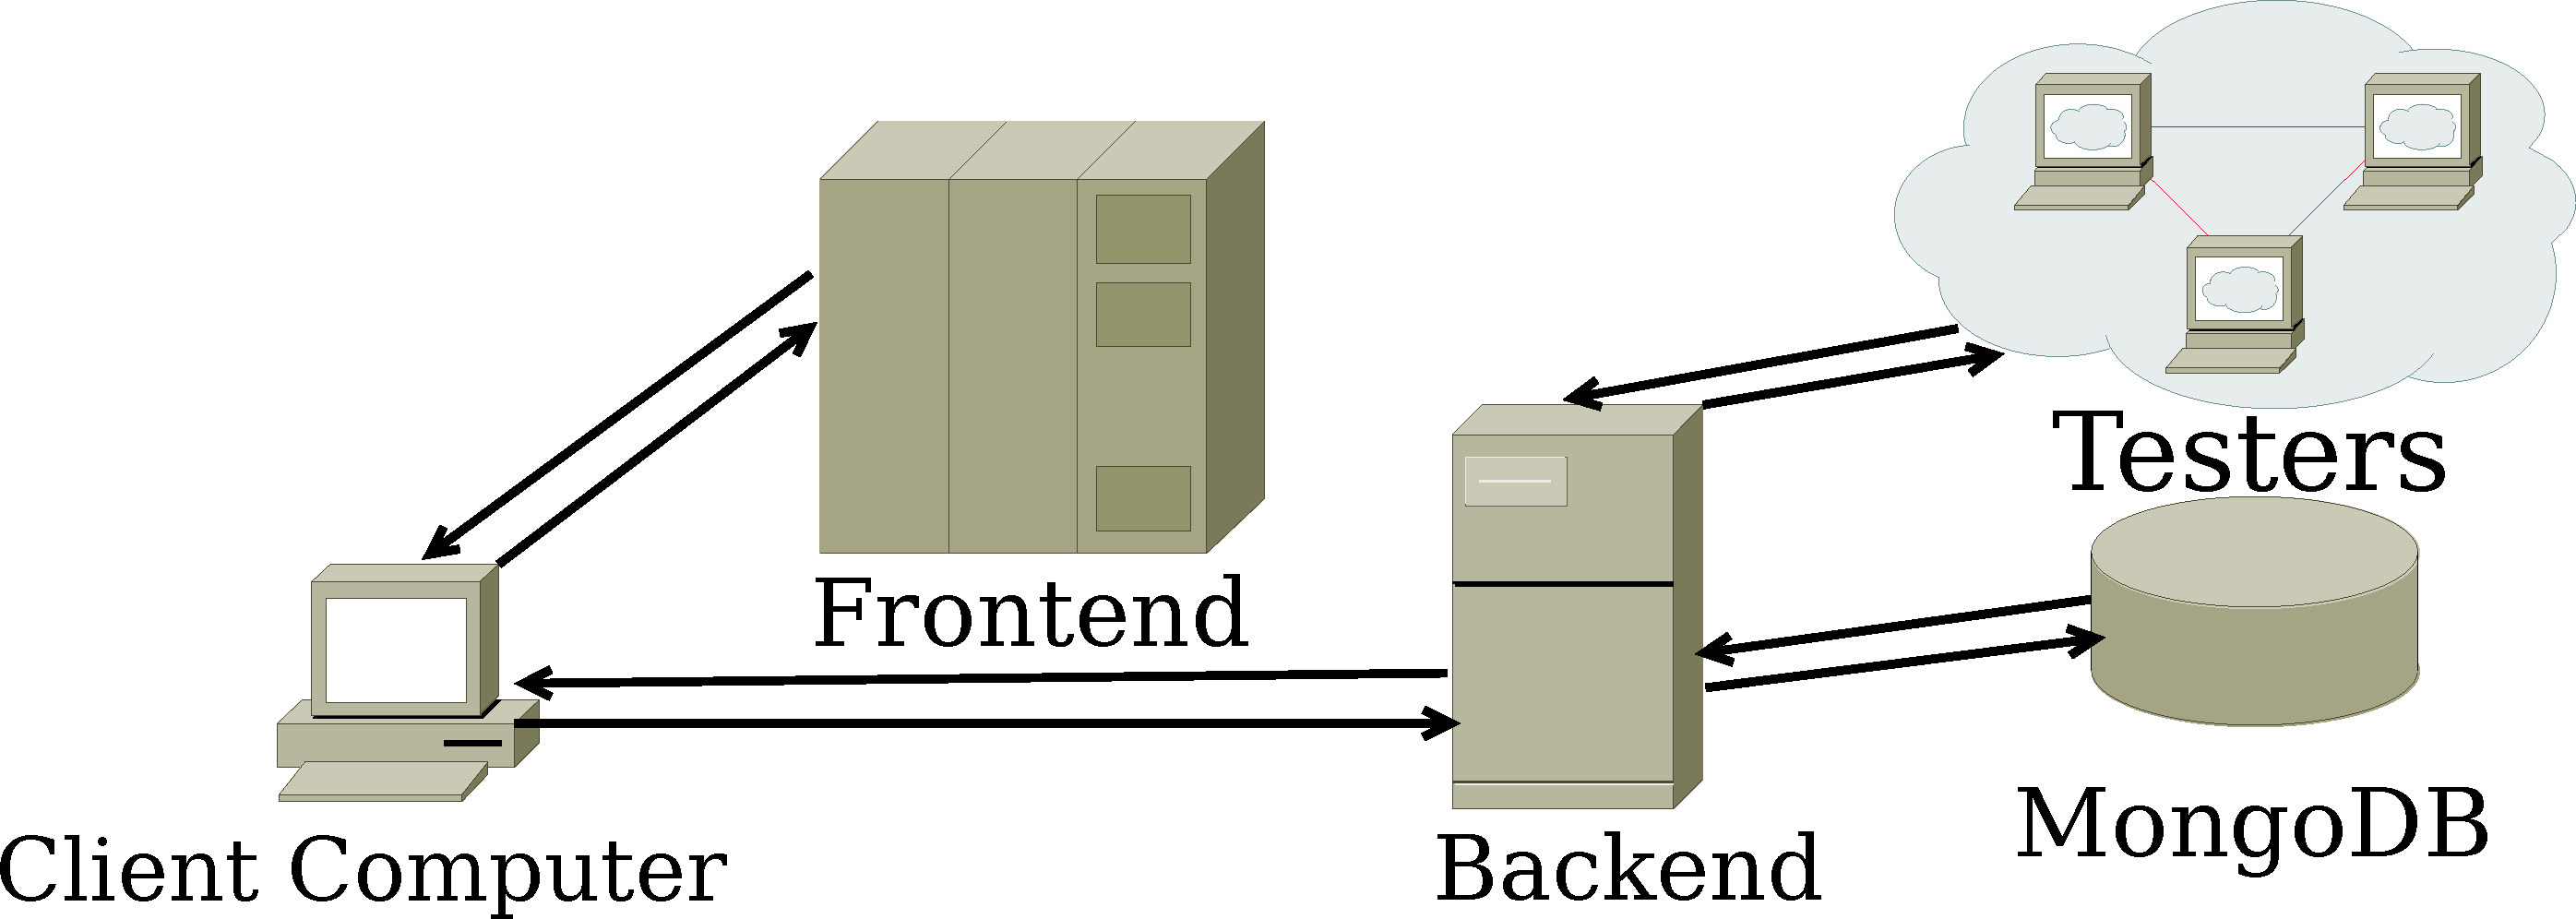
\includegraphics[width=.9\textwidth]{img/architecture.pdf}
    \caption{An overview of the architecture: First, some client interacts with the frontend, which uses javascript to send requests for resources on the backend. Then, the backend communicates with its database to serve resources. When the backend receives a request for testing, it retrieves assignment information, couples it with input data and sends it to the testers, which respond with the result of the test back through the request chain.}\label{fig:architecture}
\end{figure}

\subsection{Protocols Used}
% Protocol list
% * HTTP
% * JSON
% * Mongo Wire Protocol
% * Docker Engine
HTTPS is considered the web-standard for hypertext transport and is used to transport rendered pages as well as remote procedure calls of the website in a secure manner. It is possible to downgrade to HTTP, in case the service is to be run behind a terminating proxy, but should be run with HTTPS and valid certificates otherwise.

Object and remote procedure marshalling was done using JSON. Partially because it was native to the other tools used, meaning that any optimizations applied within the tools could be exploited, but also because it offered good readability during the debug process. Furthermore, when authenticating to CAS, the communication may be done using JSON.

For Docker communication uses a protocol on top of HTTP to facilitate container control. Since tester needs to start and stop containers remotely, this was used internally by a tester dependency.

Mongo wire protocol was used to communicate with the database, it features a simple request-response interface which was easily managed using available packages

\subsection{Flowcharts}
To visualize the interaction between the parts, some flowcharts are provided that explain the details behind some of the more common aspects of the solution. 
\begin{figure}[H]
    \centering
    \begin{subfigure}{.45\linewidth}
    \centering
    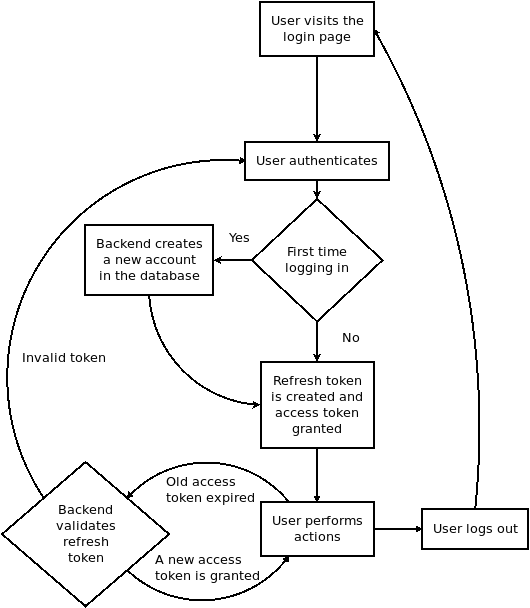
\includegraphics[width=.7\linewidth]{img/login_flowchart.png}
    \caption{An overlook of the login procedure.}
    \end{subfigure}
    %
    \begin{subfigure}{.45\linewidth}
    \centering
    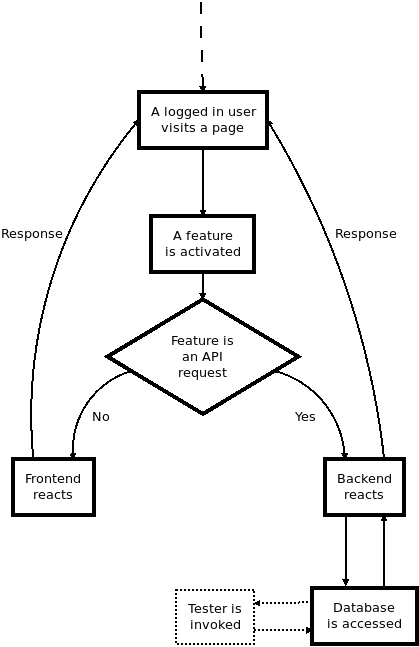
\includegraphics[width=.7\linewidth]{img/user_interaction.png}
    \caption{Continuous user interaction.}
    \end{subfigure}
    \caption{Flowcharts explaining everyday site usage.}\label{fig:common_flow}
\end{figure}
As can be seen from the flowcharts in figure~\ref{fig:common_flow}, the user either sends requests to frontend or backend, depending on what action is to be performed. Furthermore, if users are required to make API requests, scripts on the loaded website will send these requests automatically and the backend will act accordingly, performing the action if the user is logged in. Otherwise, the user will be asked to log in once more.

Since tester has some hidden complexity, an in-depth description of its workflow is provided in figure~\ref{fig:tester_internals}.
\begin{figure}
    \centering

    \begin{subfigure}{\linewidth}
    \centering
    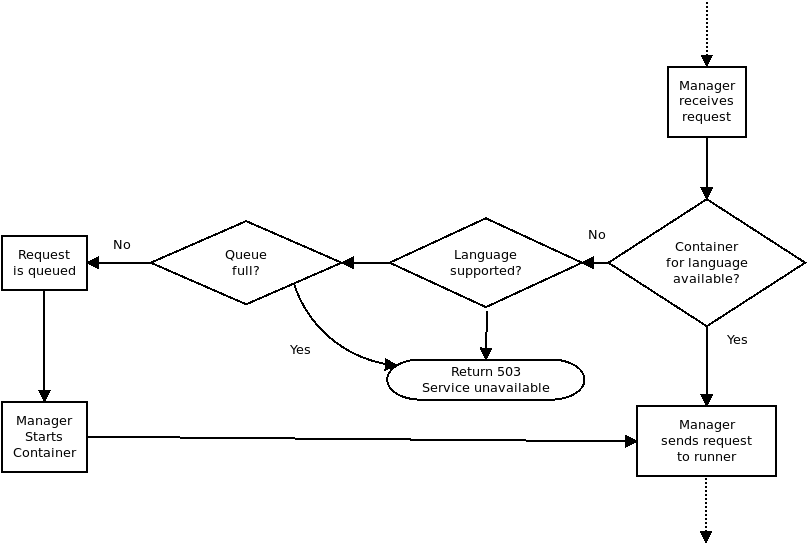
\includegraphics[width=.9\linewidth]{img/manager_usage.png}
    \caption{How manager uses runner to invoke tests.}
    \end{subfigure}
    
    \begin{subfigure}{.38\linewidth}
    \centering
    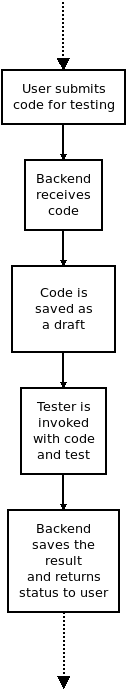
\includegraphics[width=.3\linewidth]{img/tester_usage.png}
    \caption{How backend interacts with tester.}
    \end{subfigure}
    %
    \begin{subfigure}{.6\linewidth}
    \centering
    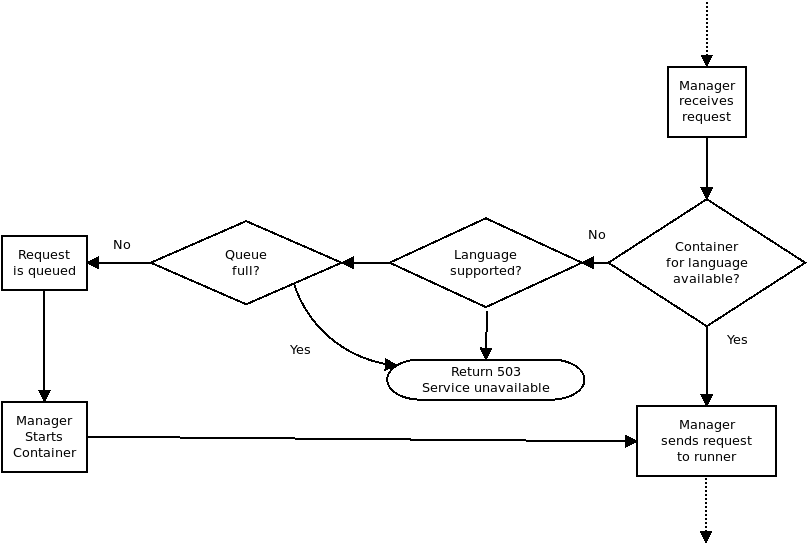
\includegraphics[width=.7\linewidth]{img/runner_usage.png}
    \caption{The internal workings of the test runner.}
    \end{subfigure}

    \caption{How tester works.}\label{fig:tester_internals}
\end{figure}
Every request generated from some outside source, such as backend or a third-party service follows the same API. There is only one endpoint that is either used as a GET to retrieve the tester status, or as POST to start a test. However, these do not always succeed as queues fill up and non-existent languages are requested. 
